%\documentclass[a4paper,fleqn,longmktitle]{cas-dc}
\documentclass[a4paper,fleqn]{cas-dc}

%\usepackage[authoryear,longnamesfirst]{natbib}
%\usepackage[authoryear]{natbib}
\usepackage[numbers]{natbib}

\newcommand{\avail}[2]{\noindent {\bf#1:}~{#2}\newline}
\newcommand{\code}[1]{\texttt{#1}}
\newcommand{\note}[1]{\emph{\color{red}{#1}}}


%%%Author definitions
\def\tsc#1{\csdef{#1}{\textsc{\lowercase{#1}}\xspace}}
\tsc{WGM}
\tsc{QE}
\tsc{EP}
\tsc{PMS}
\tsc{BEC}
\tsc{DE}
%%%

\begin{document}
\let\WriteBookmarks\relax
\def\floatpagepagefraction{1}
\def\textpagefraction{.001}
\shorttitle{Watershed Workflow}
\shortauthors{E.T. Coon}

\title [mode = title]{Watershed Workflow: a workflow for hydrologic model-data integration.}                      
\tnotemark[1]

\tnotetext[1]{BLAH BLAH BLAH US Government reserves all rights.}

\author[1]{Ethan T. Coon}[type=editor,
                      auid=000,
                      orcid=0000-0001-8124-9622]
\cormark[1]
\ead{coonet@ornl.gov}
\credit{Conceptualization, Software, Authorship}
\address[1]{Climate Change Science Institute \& Environmental Sciences Division, Oak Ridge National Laboratory, 1 Bethel Valley Road, Oak Ridge, TN, 37830, USA}
\cortext[cor1]{Corresponding author}

\author[2]{Pin Shuai}
\credit{Software}
\address[2]{Pacific Northwest National Laboratory}

\begin{abstract}
Watershed workflow does really cool stuff.
Watershed workflow does really cool stuff.
Watershed workflow does really cool stuff.
Watershed workflow does really cool stuff.
Watershed workflow does really cool stuff.
Watershed workflow does really cool stuff.
\end{abstract}

\begin{graphicalabstract}
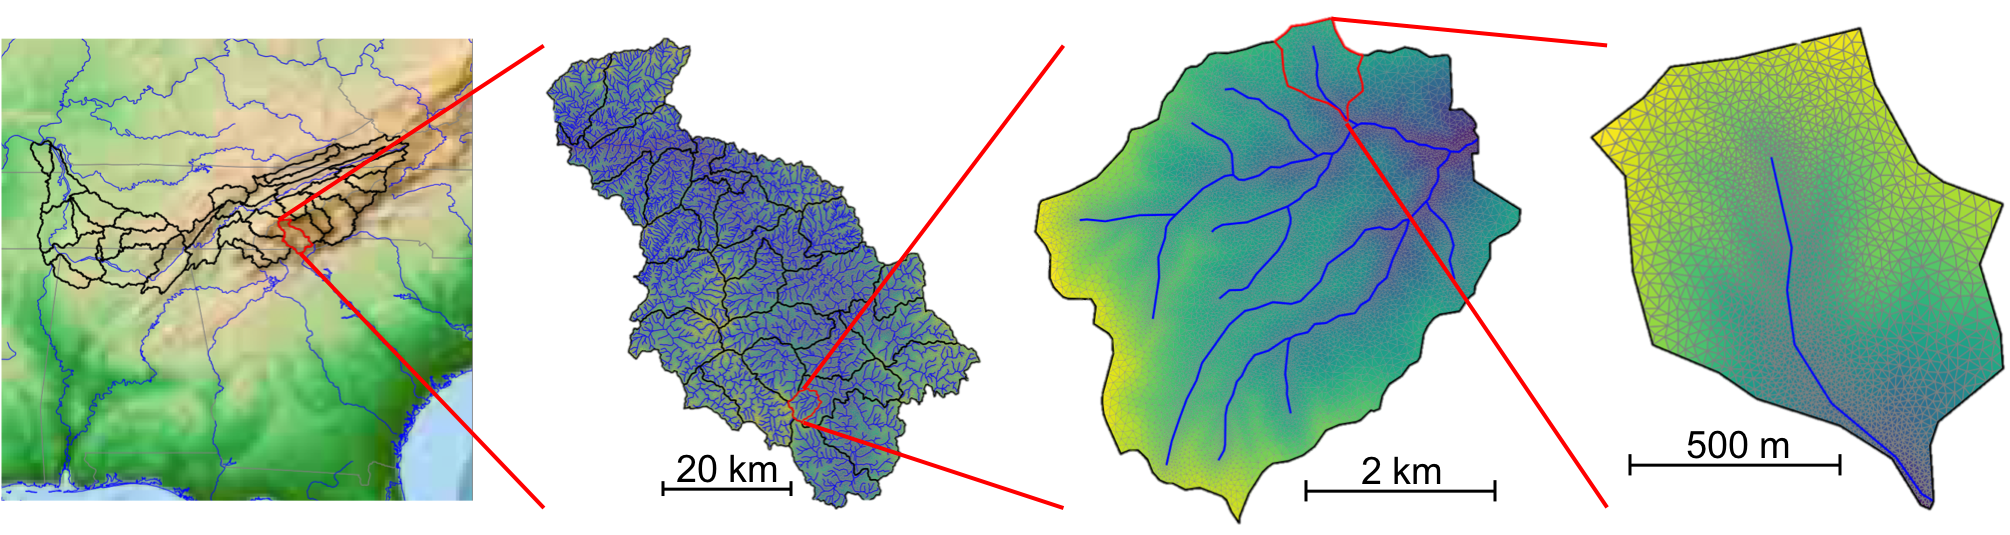
\includegraphics[width=\textwidth]{figs2/watersheds/watershed_workflow.png}
\end{graphicalabstract}

\begin{highlights}
\item Research highlights item 1
\item Research highlights item 2
\item Research highlights item 3
\end{highlights}

\begin{keywords}
integrated hydrologic modeling \sep modeling workflow \sep watershed 
\end{keywords}


\maketitle

\section*{Software availability}
%
\avail{Software name}{Watershed Workflow}
\avail{Developer}{Ethan Coon}
\avail{Year first official release}{2020}
\avail{Hardware requirements}{PC}
\avail{System requirements}{Windows, Linux, Mac}
\avail{Program language}{Python3}
\avail{Program size}{2 MB}
\avail{Availability}{\url{https://github.com/ecoon/watershed-workflow}}
\avail{License}{BSD 3-clause}
\avail{Documentation}{User guide, API documentation, and examples hosted at \url{https://ecoon.github.io/watershed-workflow}}
%
%
\section{Introduction}\label{sec:introduction}
%
\begin{itemize}
\item Integrated, distributed hydrology
\item Hyper-resolution hydro
\item remote sensing and FAIR data
\item High performance computing
\item Models are powerful but require large setup and difficult learning curve
\item Workflows and software abstractions offer opportunities to provide middleware.
\item Lit review.
\item Watershed Workflow is...
\end{itemize}

\section{Data Sources and Management}

Watershed Workflow's goal of providing a first simulation anywhere in the continental United States is made possible by a large suite of open data sources provided by US and state governmental agencies and served through many assorted web services.
Unfortunately, there is not a single source or data server for all of these, and web services differ across agencies.
Therefore, a key contribution of this library is the collection and standardization of access to many data streams in a single package.

To accomplish this, Watershed Workflow introduces the concept of a source manager, which, given a hydrologic unit code (HUC) or polygonal shape representing a watershed,
%
\begin{itemize}
\item queries, downloads, or otherwise acquires a dataset or datasets that covers that watershed,
\item unzips the file if necessary and stores the resulting files under a standardized naming convention in a data library to enable reuse,  
\item reads metadata and properties, providing shapes or rasters and metadata, and
\item does this via a standardized interface to allow users to swap data sources easily.
\end{itemize}
%
Source managers may use provided REST APIs to discover specific files to download, download files based on known URL patterns and HUCs or other indices, or directly download the data via a get/push request.
In this section we enumerate the diverse datasets needed to inform a single simulation, and describe the source manager or managers used to acquire that data.

\subsection{Watershed geometry}\label{ssc:acquisition:geom}
%
Watershed boundary datasets and hydrography datasets together form the geographic structure of a watershed.
Watershed boundary datasets are typically delineated through the analysis of elevation datasets, defining a watershed as all parts of the land surface which drain to a common point, typically in the stream network.
Watersheds are hierarchical, ranging in scale from small primary watersheds which drain into first order streams to full river basins which drain into an ocean.
In the United States, the United States Geological Survey formally calculates hydrologic units and identifies them using Hydrologic Unit Codes, or HUCs, which respect this hierarchy.
HUC 2 regions (e.g. the Upper Colorado River or the Tennessee River Basin) are the largest in areal extent, while HUC 12s, or sub-watersheds, are the smallest commonly provided, representing on the order of 100 square kilometers.
Watershed Workflow uses HUCs as an organizing unit for working with data, primarily because most datasets in the US are organized by the HUC, but also because they form physically useful domains for simulation.

Hydrography datasets provide surveys of river networks, which form the drainage network of watersheds and are where most of the fast-time scale dynamics occur.
Some hydrologic models (for instance river routing models, dam operations management models, and many flood models) directly use the river network as their simulation domain, while others (for instance the class of integrated, distributed models described here) can use the river network to refine meshes near the rivers and therefore improve resolution where fast dynamics are occuring.
Watershed boundary and Hydrography datasets are typically available as GIS shapefiles, where each watershed boundary or reach is represented as a shape.

Watershed Workflow leverages the Watershed Boundary Dataset (WBD) and the National Hydrography Dataset (NHD), USGS and EPA datasets available at multiple resolutions to represent United States watersheds.\cite{NHD}
Also used is the NHD Plus dataset, an augmented dataset built on watershed boundaries and elevation products.
By default, the 1:100,000 High Resolution datasets are used, but all resolutions are accessible through the source manager.
Data is discovered through The National Map's REST API, which allows querying for data files organized by HUC and resolution via HTTP POST requests, providing direct-download URLs.
Files are downloaded on first request, unzipped, and stored in the data library for future use.
Currently, files are indexed by 2-digit (WBD), 4-digit (NHD Plus HR) and 8-digit (NHD) HUCs.

%.. [NHD] https://www.usgs.gov/core-science-systems/ngp/national-hydrography
%.. [TNM] https://viewer.nationalmap.gov/help/documents/TNMAccessAPIDocumentation/TNMAccessAPIDocumentation.pdf

Finally, digital elevation models or digital terrain models (DEMs or DTMs, hereafter we use DEM to indicate either) are necessary to provided elevation of the ground surface.
The National Elevation Dataset and ongoing work in the USGS 3D Elevation Program (3DEP) provide rasters which cover the United States in 1-degree tiles.\cite{NED}
These data products are available at a variety of scales, but are available uniformly across the entire US at ~30m resolution and across the conterminous US at ~10m resolution.
The location and filename (which differ across the US) are discovered using The National Map's REST API and are downloaded, stitched together if needed, and returned as a single dataset and metadata profile.
Note that the above NHD, NHD+, and WBD delineations are based on data from the 3DEP program; consistent elevation maps and watershed delineations are used to ensure consistent watershed simulations.

\subsection{Land Cover}\label{ssc:acquisition:land_cover}
%
Given a watershed, surface properties are typically required to define surficial processes, including runoff through Manning's coefficient or other model parameters, evapotranspiration through leaf area index or other model inputs, and imperviousness surfaces.
Most distributed hydrologic models link these parameters to a common land cover index.
The National Land Cover Database (NLCD)\cite{NLCD} provides a map at 30m resolution of land cover across the nation at several different time slices.
This dataset is based on \note{insert sentence on satallite imagery used, etc.}
The NLCD raster is a single, ~5GB file download that covers the continental US, and additional rasters for each for Alaska, Puerto Rico, and Hawaii, hosted at static URLs.
The raster is downloaded, unzipped and stored in the data library on first request.

Watershed Workflow, in addition to standard capabilities required below, provides colormaps and labels for the various NLCD indices, allowing for plotting using standard NLCD colors.

\note{Additionally, do we want to include MODIS and LAI here?}

\subsection{Subsurface structure and properties}\label{ssc:acquisition:soil}
%
Perhaps the most important parameters required by an integrated hydrologic model are the subsurface structure and properties.
Soil horizon thicknesses, depth-to-bedrock, and soil and rock properties (e.g. permeability, porosity, and water retention curves) control the rate of infiltration, water storage, and other key processes of the water cycle.
These are also the most difficult properties to attain in standard ways across basins.
Rarely are they observable through remote sensing, leaving ground-based surveys, direct sampling, and other local measurement approaches to inform model parameters.
As a result, integrated, distributed hydrologic models have been often limited by the availability of accurate subsurface structure and parameter data.

Fortunately, synthetic, aggregated datasets of soil structure and properties are becoming more common, and, at least for the top few meters of soil, are relatively well constrained.
Depth-to-bedrock and deeper information is correspondingly harder to find, but global products are available.
Modelers must choose both what products to build from, and also at what resolution and structural complexity.
Reasonable modeling studies might choose simple models and few parameters, or complex models with varying horizon thicknesses and properties, as fits the modeling question being asked.

For instance, products intended for Earth System Models such as GLobal HYdrology MaPS version 2.0 (GLHYMPS)\cite{huscroft2018compiling} provide coarse resolution information of aggregated properties, providing a single porosity and permeability for all soil above the bedrock.
\note{GLHYMPS description sentence, what is it, etc.}

GLHYMPS is available through a data DOI\cite{}, but requires a web form to be completed; out of respect to the author, we therefore require users to manually download this dataset rather than bypassing the form.
While GLHYMPS is complete in the information in provides, it not sufficient, as it does not include water retention curves through van Genuchten or other parameters.

More detailed survey products such as the US National Resources Conservation Service's web soil survey (SSURGO and STATSGO2) datasets provided detailed information.
These products are based on extensive US and State Geological Surveys, and cover the entirety of the conterminous US.
Soil survey files identify a set of map unit shapefiles that cover the ground, identifying multiple components of the soil in each map unit and multiple soil horizons in each component.
The soil survey includes porosity, permeability, bulk density, and sand, silt, and clay compositional percentages for several horizons in each component.
Watershed Workflow provides tools to average these values, both vertically across horizons and then horizontally across components by area fraction, to determine a single set of properties for each map unit.
Note that permeabilities are averaged in log-space.
Then, Watershed Workflow wraps the Rosetta version 3-beta\cite{} model for pedotransfer functions, allowing the calculation of water retention curves in the form of van Genuchten parameters\cite{}.

The NRCS Web Soil Survey provides several ways to access its data.
Here we leverage the SQL-based query structure of the provided web tools\cite{}.
These allow users to post requests based on a bounding box of the area of interest, downloading collections of shapefiles that include map-unit keys.
These files, along with corresponding SQL queries for soil properties by map-unit key, are saved to disk and potential used to color a raster.
We note that the (gridded) gSSURGO product is available by state -- this product, while potentially useful to users, is served in a cloud-based service whose software toolkit packages require purchased access.
While a user may manually click through links to download gSSURGO, it is not possible for an automated workflow to discover the URL, meaning that the REST API is more robust for an automated application.
Watershed Workflow does allow the use of gSSURGO files, but the user must download them manually.
While these datasets are some of the best information available, the dataset as a whole is limited to the top two meters and is not complete in that some formations do not have sufficient data to infer all needed soil properties.

In many watersheds, individual soil pits or boreholes might provide extremely detailed information in exchange for being localized in space; individual users should incoporate this data where possible.

Here, following with the general concept of Watershed Workflow, we provide a default dataset available everywhere, but also provide the ability to use other datasets as chosen by the user.
\note{Can we provide a single default?  A composite default?  Or is user intervention required here?}
In this way, we can ensure that there is a well-posed problem that can be automatically formed everywhere in the continental US.
However, this may be either too complex (by introducing too many free parameters for calibration, for instance) or too simple (by not considering important fractured bedrock or other subsurface formations) for a given modeling study.
Therefore, we emphasize that it is crucial for a given study to choose subsurface structure and properties carefully, and understand the sensitivity of their result to these choices.

\subsection{Meteorological data}\label{ssc:acquisition:met}
%
Given surface and subsurface structural data and properties, the crucial remaining model input is meteorological data, typically including precipitation, air temperature, relative humidity, and radiation fluxes.
These variables are used to drive the transient conditions of a hydrologic model, determining water sources and sinks (e.g. precipitation, evapotranspiration, etc).
DayMet\cite{} provides daily meteorological data at 1 km resolution across the entirety of North America.
It curates and synthesizes daily weather stations datasets from the Global Historical Climate Network Daily Database \cite{}, then bias corrects as needed, and spatially and temporally interpolates to create the resulting gridded product.

Given the model domain, Watershed Workflow leverages the DayMet REST API services to download, for each year and variable, a file containing all pixel values in a bounding box covering the model domain.
The library then merges these into a single file for use by the model code.
This is typically preferred to interpolating the gridded product directly onto the mesh due to file size concerns.
A hyperresolution simulation may consist of millions of surface cells; saving a data point for every cell at every day of a given simulation may be prohibitively expensive.
Instead, it is expected that the interpolation on the mesh can be handled inside of a simulator from the raster.


\subsection{User-provided data}\label{ssc:acquisition:user}
%
Finally, it is recognized that these data products, while sufficient to generate a first model, may not be the first choice for a given watershed, problem, or resolution.
In addition to being designed to be extensible (see Section \ref{sec:approach}), generic source managers are provided for using user-provided files, including both shapefile-based products and raster-based products.
These files can be loaded and curated for use in the workflow using the source-agnostic tools below.

\section{Data Curation}\label{sec:data_curation}
%
Each of the above data products must be standardized and placed on a common mesh for use in a hydrologic model.
Watershed Workflow leverages a variety of open source libraries to accomplish this goal, and provides functionality to chain the workflow across these tools.

\subsection{Coordinate Reference System transformation and standardization}
%
Each dataset is provided in its own coordinate reference system (CRS), as described by either Well-Known-Text (WKT) format strings or EPSG Geodetic Parameter Dataset code.
Furthermore, most geospatial tools in python seem to provide their own solution for interacting with these objects.
Watershed Workflow uses the \code{proj4} python library's CRS as its underlying CRS object, and provides functions for converting this object to objects used by a variety of other python libraries, including \code{fiona}, \code{rasterio}, and \code{cartopy}.
It then provides a series of wrappers to the \code{proj4} library to change the coordinate system of both shapes and raster objects.

Users can choose to work in whichever CRS makes the most sense for their watershed, but typically it is recommended to use the CRS of the meteorological dataset.
This is because interpolating from the meteorological data raster onto the unstructured mesh is much more computationally efficient if the mesh and the meteorological data are in the same coordinate system.

\subsection{Domain Manipulation and Scale Transformation}
%
While boundary domain and hydrography datasets are available from a variety of sources, these domains may or may not be appropriate for direct simulation.
A key consideration is scale.
Watershed Workflow wraps a variety of tools to manipulate the domain of interest, frequently coarsening it from higher resolution to the resolution desired by the user.
Additionally, tools are provided to filter and smooth rasters, allowing high resolution rasters to be restricted to the mesh cells in a variety of ways.

Watershed boundaries and river reaches are loaded from shapefiles into a list of polygons and polylines, respectively.
Polygons are loaded into a split data structure, where overlapping HUC boundaries are combined into collections of LineStrings.
This allows the topological and geometric manipulation of these shapes to guarantee consistency of boundaries between HUCs, ensuring that geometric transformations cannot lose or gain area (See Figure \ref{fig:split_hucs}).

Reaches are processed into a list of tree-based data structures, with one for each outlet which terminates on or within the watershed boundary.
While a tree assumes that rivers only merge as they move downstream, we have found this to be sufficient (despite implications for high resolution data in braided stream networks).
Optionally, river networks are pruned if they include too few reaches or do not exit the watershed -- this is possible in the case of man-made irrigation canals and other corner cases.
From the tree network, it is straightforward to accumulate and analyze river network properties from reach properties provided by the dataset, such as accumulated drainage area or other values; these may be used in a workflow to prune or otherwise change the network.

Given these data structures, a user may wish to coarsen from the native resolution to a resolution more tractable for simulation.
As an example, NHDPlus datasets provide watershed boundaries whose shapes consist of points that are often within $10\,m$ of each other.
Using this shape to generate a mesh would result mesh elements that include edges of that same size; this is typically too small to be computationally feasible for simulation.
Both watershed boundaries and river networks may be simplified, using \code{shapely}'s standard GIS-based \code{simplify} algorithm, coarsening the typical edge length.
This is done in a way to ensure that the HUCs still partition the domain, not allowing overlap or disjoint shapes.
Similarly, river networks are simplified in a way that preserves the topological relationships (intersections) of rivers and HUC boundaries.

Additionally, many raster images are now available at 30m or higher resolution, but this is too high for even hyperresolution simulations.
Algorithms are wrapped in a standard interface to resample the domain onto a coarser raster; some of these are provided from \code{rasterio} (nearest-neighbor, median, etc) and others are provided from \code{scipy} (Gaussian filters and other image processing filters).
Finally, a simple unstructured pit-filling algorithm is provided once a DEM has been mapped onto an unstructured mesh.

\subsection{Mesh Generation}
%
Given a watershed boundary and a DEM on that boundary, a mesh must be formed to cover that domain for use by distributed hydrologic models.
As the primary target code considered here is an unstructured code, we leverage the \code{Triangle} library\cite{} to triangulate the map-view surface.
Triangle forms Delaunay triangulations which are preferred for simulation accuracy, and allow user-provided refinement functions through the \code{meshpy} library which is used to call \code{Triangle} (a C code) from python.
A variety of standard functions are provided, including options for refining by triangle area, minimum angle, and distance from the river network.
The river network may be directly included within the mesh, ensuring that the network exists as edges in the mesh, or may be used solely to refine the triangles in the river corridor.

While optimal meshes for simulation are an area of active research\cite{ozgur2020??}, it is common to refine the mesh near the river network.
This results in higher resolution where faster dynamics are occuring, and decreases the minimum stream width resolved in an integrated simulation.
An example mesh resulting from this workflow is seen in Section \ref{sec:example}.

\subsection{Plotting}
%
Finally, we find it is crucial to be able to visualize these watershed products effectively.
With such complicated workflows, data products, and geographic information, quality imagery makes it much easier for both model users and stakeholders to understand and internalize model results.
Watershed Workflow provides a large collection of plotting utilities and that leverage \code{matplotlib}\cite{} for base plotting capability and \code{cartopy} to ensure watersheds are plotted accurately in their native CRS projection and to provide underlying basemaps for geographic and political boundaries.
Defaults and standard styles are used to ensure efficient communication of this information across watersheds and model simulations.

\section{Software Design}\label{sec:approach}
%
\begin{itemize}
\item Python libraries for code, Jupyter notebooks for orchestration
\item Installation from Anaconda packages
\item ReST APIs and open data portals allow automatic dataset discovery.
\end{itemize}

\section{A worked example: the Coweeta Hydrologic Laboratory}\label{sec:example}
%
To motivate each aspect of the workflow, it is useful to consider a worked example throughout the text of this manuscript.
In the rest of the paper we provide a complete example, demonstrating the datasets and concepts needed to provide a complete simulation.
The simulation is based on the Coweeta Hydrologic Laboratory, a US National Forest Service station in the US Southeast,\cite{??} and results are shown from the Advanced Terrestrial Simulator\cite{CoonWRR??} (ATS), an integrated, distributed hydrologic model based on unstructured meshes.
Note that the complete Jupyter notebook used to define this example is provided in supplementary material, and is maintained and updated with new versions in the Watershed Workflow repository and documentation.

As input to the process, a shapefile defining the boundary of the Coweeta domain is assumed provided by the user.
Note that this could equivalently be a USGS Hydrologic Unit Code (HUC), and the boundary would be downloaded within the workflow.

\section{Conclusions and Future Work}\label{sec:conclusions}

\printcredits

\bibliographystyle{cas-model2-names}
\bibliography{refs}


%\vskip3pt

\bio{figs2/bio/coon.jpg}
Dr. Ethan Coon is a computational hydrologist in the Climate Change Science Institute at ORNL.
He has a background in applied and computational mathematics, and has done research in applying computational methods for the Earth, especially land surface and subsurface processes.
Broadly he is interested in process-based modeling, integrating models with data, and leverage modeling to understand the processes that govern our changing planet.
\endbio


\end{document}

